\chapter{Konzeption des Modells}
\label{chap:konzept}

\section{Datensatz}

\label{chap:3-Datensatz}
Analog zu der in Kapitel \ref{chap:vorherige-arbeiten-rub} beschriebenen Arbeit verwendet diese Studienarbeit den \ac{GTSRB} als Datensatz. Dass dies mit 39.209 Bildern der größte veröffentlichte Datensatz für deutsche Straßenschilder ist, stellt hierbei den ausschlaggebenden Punkt dar.

Die Bilder des \ac{GTSRB} verteilen sich auf 43 Klassen respektive 43 verschiedene Arten von Straßenschildern. Eine Auflistung aller Klassen ist im Anhang in Abbildung \ref{fig:all-pictograms} dargestellt. Beispielbilder aus dem \ac{GTSRB} zeigt Abbildung \ref{fig:gtrsb-paper-bsp-images}. \cite{GTSRB}


\begin{figure}[H]
   \centering
   \begin{subfigure}[b]{0.125\textwidth}
       \centering
       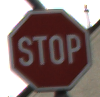
\includegraphics[height=\textwidth]{../images/GTSRB/00093.png}
       \caption{}
       \label{fig:gtrsb-paper-bsp-image-1}
   \end{subfigure}
   \hspace{3em}%
   \begin{subfigure}[b]{0.125\textwidth}
       \centering
       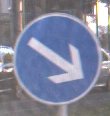
\includegraphics[height=\textwidth]{../images/GTSRB/00847.png}
       \caption{}
       \label{fig:gtrsb-paper-bsp-image-2}
   \end{subfigure}
   \hspace{3em}%
   \begin{subfigure}[b]{0.125\textwidth}
       \centering
       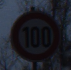
\includegraphics[height=\textwidth]{../images/GTSRB/00040.png}
       \caption{}
       \label{fig:gtrsb-paper-bsp-image-3}
   \end{subfigure}
   \hspace{3em}%
   \begin{subfigure}[b]{0.125\textwidth}
    \centering
    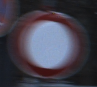
\includegraphics[height=\textwidth]{../images/GTSRB/00052.png}
    \caption{}
    \label{fig:gtrsb-paper-bsp-image-4}
\end{subfigure}
      \caption{Beispielbilder aus dem \acs{GTSRB} Datensatz \cite{GTSRB}}
      \label{fig:gtrsb-paper-bsp-images}
\end{figure}

Der \ac{GTSRB} setzt sich aus Bildern zusammen, die unterschiedliche Seitenverhältnisse und verschiedene Auflösungen besitzen. Ein Großteil davon ist kleiner als 100x100 Pixel. Auf jedem Bild ist genau ein Straßenschild zu sehen. Die Bilder basieren auf Videos, die durch die Autoren tagsüber im Straßenverkehr aufgenommen wurden. Dabei sind die Trainingsbilder ungleich auf die Anzahl an Klassen verteilt. Dies hängt mitunter damit zusammen, dass die jeweiligen Schilder nicht gleich häufig im Straßenverkehr vorkommen. Zusätzlich zu den Trainingsbildern besitzt der \ac{GTSRB} 12.630 Testbilder, welche in dieser Arbeit zur Evaluation des Modells verwendet werden können. Eine nennenswerte Eigenschaft des \ac{GTSRB} ist, dass eine signifikante Anzahl an Bildern einer Klasse sich ähnlich sehen. Das hängt damit zusammen, dass sie mit zeitlicher Verzögerung aus der selben Fahrsituation stammen. \cite{GTSRB}

Die Bilder, die durch diese Studienarbet generiert werden sollen, haben eine Auflösung von 256x256 Pixel. Auf den genauen Hintergrund hierzu wird zu einem späteren Zeitpunt eingegangen. Unter anderem deshalb ist der \ac{GTSRB} für diese Arbeit zunächst so präpariert, dass nur Bilder verwendet werden, die mindestens 50 Pixel breit oder hoch sind. Dies wird im Verlauf geändert, sodass die Mindestgröße 75 Pixel beträgt. Das verringert die Anzahl an verfügbaren Trainingsbildern signifikant. Der präparierte Datensatz besteht aus 4.510 Bildern, wodurch nur etwa 11\% des \ac{GTSRB} genutzt werden.

Die Verteilung der Daten ist auch im präparierten Datensatz nicht homogen. Das nachfolgende Diagramm zeigt hierfür die Anzahl an Trainingsbildern pro Klasse.

\definecolor{plotcolor}{HTML}{2b2b2b}
\definecolor{Aufhebungen}{HTML}{58508d}
\definecolor{Verbotszeichen}{HTML}{bc5090}
\definecolor{Gefahrzeichen}{HTML}{ff6361}
\definecolor{Einzigartig}{HTML}{ffa600}
\definecolor{Richtungsweiser}{HTML}{444e86}
\definecolor{Geschwindigkeitsbegrenzungen}{HTML}{003f5c}

\definecolor{chinesedata}{HTML}{009F93}
\definecolor{mapillary}{HTML}{FF6542}

%\begin{figure}[H]
%    \centering
%    \begin{tikzpicture}
%        \begin{axis} [ybar, ylabel={Absolute Häufigkeit}, xlabel={Klassen-ID}, width=\linewidth*0.9, height=\linewidth*0.3, scale only axis=true, xmin=-1, xmax=43, ymin=0, ymax=450, bar width=0.2cm, ytick={0, 100, 200, 300, 400},
%            symbolic x coords={
%                -1, 0, 1, 2, 3, 4, 5, 6, 7, 8, 9, 10, 11, 12, 13, 14, 15, 16, 17, 18, 19, 20, 21, 22, 23, 24, 25, 26, 27, 28, 29, 30, 31, 32, 33, 34, 35, 36, 37, 38, 39, 40, 41, 42, 43}
%        ]

        % x+0.4
%        \addplot[Geschwindigkeitsbegrenzungen, fill] coordinates {
%            (0, 36)
%            (1, 312) 
%            (2, 184)
%            (3, 102) 
%            (4, 150)
%            (5, 84)
%            (7, 80)
%            (8, 52)
%        };
        % x-0.45
%        \addplot[Aufhebungen, fill] coordinates {
%            (6, 13)
%            (32, 10) %(17, 21)
%            (41, 14)
%            (42, 5)
%        };
        % x - 1
%        \addplot[Verbotszeichen, fill] coordinates {
%            (9, 141)
%            (10, 73)
%            (16, 71)
%            (17, 20)
%        };
%        \addplot[Gefahrzeichen, fill] coordinates {
%            (11, 301)
%            (18, 279) %(26, 118)
%            (19, 45) %(27, 62)
%            (20, 24) %(28, 126)
%            (21, 51) %(29, 60)
%            (22, 45) %(30, 71)
%            (23, 112) %(31, 117)
%            (24, 40) %(6, 14)
%            (25, 341) %(9, 214)
%            (26, 88) %(10, 110)
%            (27, 29) %(12, 424)
%            (28, 93) %(13, 534)
%            (29, 42) %(14, 269)
%            (30, 63) %(15, 77)
%            (31, 93) %(16, 85)
%        };
%        \addplot[Einzigartig, fill] coordinates {
%            (12, 306) %(20, 31)
%            (13, 405) %(21, 70)
%            (14, 203) %(22, 58)
%            (15, 53) %(23, 144)
%        };
%        \addplot[Richtungsweiser, fill] coordinates {
%            (33, 94) %(32, 12)
%            (34, 33) %(33, 116)
%            (35, 90)
%            (36, 23)
%            (37, 28)
%            (38, 148)
%            (39, 66)
%            (40, 68)
%        };
%        \end{axis}
%    \end{tikzpicture}
%    \caption{Häufigkeitsverteilung der Klassen von Straßenschildern im präparierten \ac{GTSRB}}
%    \end{figure}

\begin{figure}[H]
    \centering
    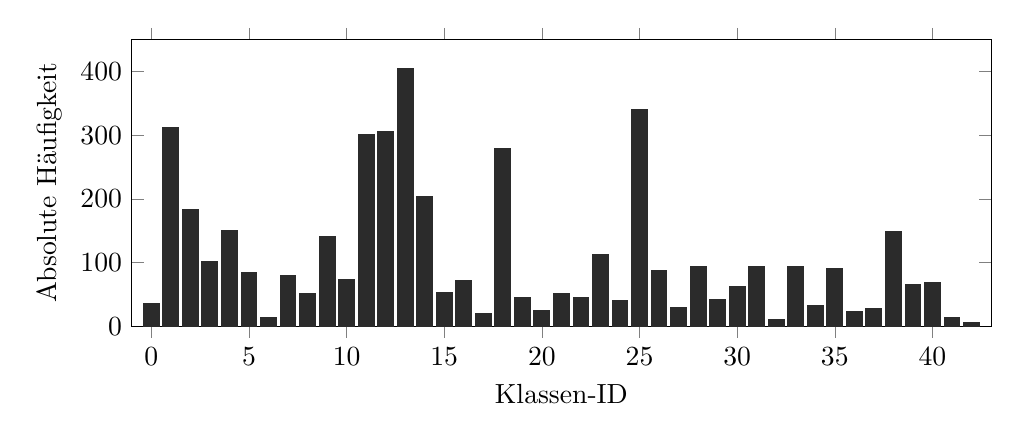
\begin{tikzpicture}
        \begin{axis} [ybar, ylabel={Absolute Häufigkeit}, xlabel={Klassen-ID}, width=\linewidth*0.9, height=\linewidth*0.3, scale only axis=true, xmin=-1, xmax=43, ymin=0, ymax=450, bar width=0.2cm, ytick={0, 100, 200, 300, 400}]
        \addplot[plotcolor, fill] coordinates {
            (0, 36) %(0, 40)
            (1, 312) %(1, 390) 
            (2, 184) %(2, 270)
            (3, 102) 
            (4, 150) %(3, 127)
            (5, 84) %(4, 192)
            (6, 13) %(5, 113)
            (7, 80) %(7, 101)
            (8, 52) %(8, 69)
            (9, 141) %(11, 396)
            (10, 73) %(18, 342)
            (11, 301) %(19, 56)
            (12, 306) %(20, 31)
            (13, 405) %(21, 70)
            (14, 203) %(22, 58)
            (15, 53) %(23, 144)
            (16, 71) %(24, 75)
            (17, 20) %(25, 451)
            (18, 279) %(26, 118)
            (19, 45) %(27, 62)
            (20, 24) %(28, 126)
            (21, 51) %(29, 60)
            (22, 45) %(30, 71)
            (23, 112) %(31, 117)
            (24, 40) %(6, 14)
            (25, 341) %(9, 214)
            (26, 88) %(10, 110)
            (27, 29) %(12, 424)
            (28, 93) %(13, 534)
            (29, 42) %(14, 269)
            (30, 63) %(15, 77)
            (31, 93) %(16, 85)
            (32, 10) %(17, 21)
            (33, 94) %(32, 12)
            (34, 33) %(33, 116)
            (35, 90) %(34, 39)
            (36, 23) %(35, 121)
            (37, 28) %(36, 53)
            (38, 148) %(37, 31)
            (39, 66) %(38, 195)
            (40, 68) %(39, 87)
            (41, 14) %(40, 88)
            (42, 5) %(41, 19)
                     %(42, 10)
        };
        \end{axis}
    \end{tikzpicture}
    \caption{Häufigkeitsverteilung der Klassen von Straßenschildern im präparierten \ac{GTSRB}}
    \end{figure}

Eine ungleiche Verteilung der Trainingsdaten kann die Qualität der generierten Bilder negativ beeinflussen. Die in Kapitel \ref{chap:vorherige-arbeiten-rub} beschriebene Veröffentlichung gibt hierauf bereits Hinweise \cite{gtsrbGAN}. Aus diesem Grund, und da die Größe des präparierten Datensatzes als zu gering bewertet werden kann, ist der Datensatz derart erweitert, dass er einerseits mehr Trainingsbilder enthält und andererseits eine gleichmäßigere Verteilung der Klassen vorliegt. Dabei wird nicht darauf geachtet, jede einzelne Klasse möglichst gleich oft zu repräsentieren, sondern jede Kategorie von Klassen. Die 43 Klassen werden dazu in die Kategorien \emph{Geschwindigkeitsbegrenzungen}, \emph{Richtungsweiser}, \emph{Aufhebungen}, \emph{Verbotszeichen}, \emph{Gefahrzeichen} und \emph{Einzigartig} unterteilt. Es zeigt sich nämlich, dass das Modell zwischen Straßenschildern, die eine ähnliche Bedeutung und damit auch äußerliche Ähnlichkleiten besitzen, recht gut transferieren kann. Diese Einteilung der Schilder in unterschiedliche Kategorien erfolgt auch in der ursprünglichen Veröffentlichung des \ac{GTSRB}. Die Kategorisierung für diese Studienarbeit ist identisch, verwendet jedoch deutschen Bezeichnungen für die Kategorien. Im Anhang befindet sich eine übersicht über die Kategorien von Schildern und ihre zugeordneten Klassen.

Der Großteil an hinzugefügten Trainingsdaten stammt aus der chinesischen \emph{Traffic Sign Recognition Database}, die ein Teil der \emph{Chinese Traffic Sign Database} ist. Dieser Datensatz ist bedeutend kleiner als der \ac{GTSRB}, bietet jedoch auch einige Bilder mit einer höheren Auflösung als der \ac{GTSRB}. Somit ist  hier ein größerer Anteil des Datensatzes nutzbar. Allgemein ähneln diese Bildern denen des \ac{GTSRB}. Mit dem Unterschied, dass sie chinesische Straßenschilder zeigen. Für den präparierten Datensatz werden nur die Bilder verwendet, die in eine der genannten Kategorien fallen. Nachfolgend sind Beispielsbilder aus dem Datensatz dargestellt: \cite{chinese-dataset}


\begin{figure}[H]
    \centering
    \begin{subfigure}[b]{0.125\textwidth}
        \centering
        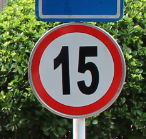
\includegraphics[height=\textwidth]{../images/3 Konzeption des Generative Adversarial Networks/Chinese Dataset/001_0013.png}
        \caption{}
    \end{subfigure}
    \hspace{3em}%
    \begin{subfigure}[b]{0.125\textwidth}
        \centering
        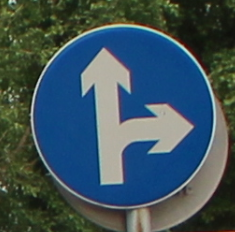
\includegraphics[height=\textwidth]{../images/3 Konzeption des Generative Adversarial Networks/Chinese Dataset/020_0005.png}
        \caption{}
    \end{subfigure}
    \hspace{3em}%
    \begin{subfigure}[b]{0.125\textwidth}
        \centering
        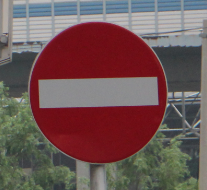
\includegraphics[height=\textwidth]{../images/3 Konzeption des Generative Adversarial Networks/Chinese Dataset/055_1_0029.png}
        \caption{}
    \end{subfigure}
    \hspace{3em}%
    \begin{subfigure}[b]{0.125\textwidth}
     \centering
     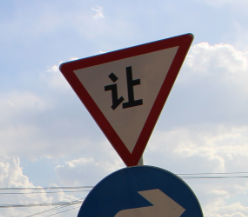
\includegraphics[height=\textwidth]{../images/3 Konzeption des Generative Adversarial Networks/Chinese Dataset/056_1_0015.png}
     \caption{}
 \end{subfigure}
       \caption{Beispielbilder aus der chinesischen Traffic Sign Recognition Database \cite{chinese-dataset}}
       \label{fig:chinese-dataset-bsp-images}
 \end{figure}

Zu sehen ist in Abbildung \ref{fig:chinese-dataset-bsp-images} eine Geschwindigkeitsbegrenzung, ein Richtungsweiser, ein Verbotszeichen und ein Schild der Kategorie \emph{Einzigartig}. Der präparierte Datensatz beinhaltet auch Schilder, die nicht durch das Modell dieser Studienarbeit generiert werden sollen. Wie etwa die in Abbildung \ref{fig:chinese-dataset-bsp-images} vorhandene Geschwindigkeitsbegrenzung von 15$\frac{km}{h}$. Die Idee ist, dass das Modell diese Bilder dennoch nutzen kann, um die Generierung von anderen Geschwindigkeitsbegrenzungen zu optimieren. Es sind allgemein Unterschiede zu deutschen Straßenschildern vorhanden, die jedoch in dieser Arbeit als vernachlässigbar angenommen werden. Zumindest dann, wenn deutsche Straßenschilder weiterhin den größten Teil des präparierten Datensatzes ausmachen. Eine gewisse Ähnlichkeit ist vorhanden, auch da das Aussehen von Straßenschildern durch das Wiener Übereinkommen über Straßenverkehrszeichen in vielen Ländern weltweit vereinheitlicht ist \cite{vienna-convention}. \cite{chinese-dataset}

Zusätzlich setzt sich der präparierte Datensatz aus Bildern weiterer Datensätze zusammen. Hier ist jedoch die Anzahl an Bildern signifikant geringer als die der chinesischen Traffic Sign Recognition Database. Zwei der Datensätze bestehen aus Bildern, die eine vollständige Sicht außerhalb des Fahrzeugs zeigen. Hier sind demnach gegebenenfalls mehrere Straßenschilder pro Bild zu sehen, wobei zusätzlich andere Fahrzeuge, Gebäude, Personen und weitere Objekte sichtbar sind. Die Datensätze nennen sich \emph{Mapillary Traffic Sign Dataset} und \emph{BelgianTS Dataset} \cite{dataset-mapillary} \cite{dataset-belgiants}.

\begin{figure}[H]
    \centering
    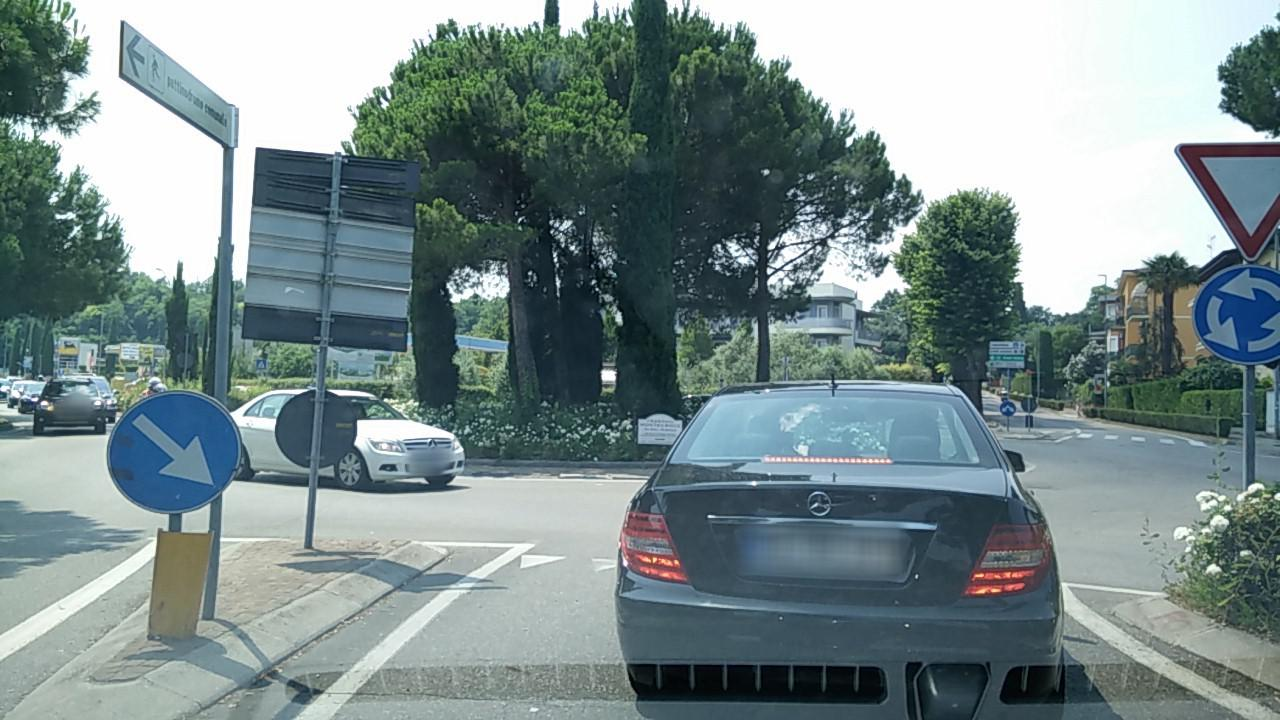
\includegraphics[height=0.3\textwidth]{../images/3 Konzeption des Generative Adversarial Networks/mapillary.jpg}
    \caption{Beispielbild aus dem \emph{Mapillary} Datensatz \cite{dataset-mapillary}}
    \label{fig:full-mapillary-image}
\end{figure}

Da diese Bilder manuell so zugeschnitten werden müssen, dass sie ähnlich zu dem \ac{GTSRB} und der chinesischen Traffic Sign Recognition Database einzelne Schilder mit wenig Hintergrund zeigen, macht diese Menge an Bildern einen geringeren Anteil aus. Aus einem dritten Datensatz werden weniger als 50 Bilder verwendet \cite{dataset-make-ml}. Hier sind größtenteils Stopschildern zu sehen mit einer Bildauflösung von etwa 190 bis zu 300 Pixel in der Höhe oder Breite.

Für diese Studienarbeit existiert ein Ordner \mintinline{python}|data|, der alle für die Arbeit relevanten Bilddateien enhält. Der Ordner ist öffentlich unter \href{https://drive.google.com/drive/folders/1310Eb5WDgaszu47k6V8St5m-QtQV1Ocg?usp=sharing}{\textbf{diesem Link}} verfügbar (Stand: 09.06.2023). In dem Unterordner \mintinline{python}{Train} befindet sich dort der gesamte Trainingsdatensatz.

Nachfolgende Abbildung zeigt die Häufigkeitsverteilung dieser Trainingsdaten (x-Achse) je Straßenschild-Kategorie (y-Achse). Die drei letztgenannten Datensätze sind in der Farbkodierung der Kategorie \emph{Sonstige} zugeordnet.

\begin{figure}[H]
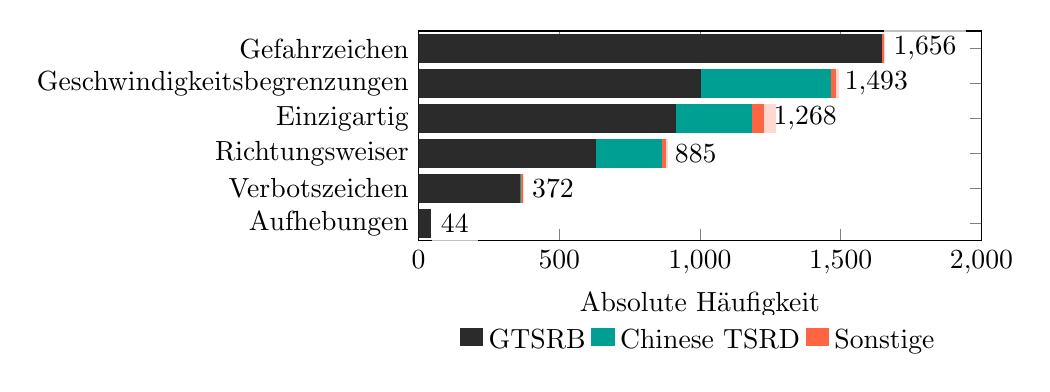
\begin{tikzpicture}
\begin{axis}[ 
xbar stacked, xmin=0, height=\linewidth*0.35, width=\linewidth*0.72,
xlabel={Absolute Häufigkeit},
legend style={at={(0.5,-0.350)}, anchor=north,legend columns=-1, draw=none},
symbolic y coords={
    Aufhebungen, 
    Verbotszeichen,
    Richtungsweiser,
    Einzigartig,
    Geschwindigkeitsbegrenzungen,
    Gefahrzeichen,
    },
ytick=data,
%nodes near coords, 
%nodes near coords align={horizontal},
ytick=data, xmax=2000, xtick={0, 500, 1000, 1500, 2000}
]
\addplot+[plotcolor, fill] coordinates {
    (914,Einzigartig)
    (1000,Geschwindigkeitsbegrenzungen) 
    (630,Richtungsweiser)
    (42,Aufhebungen)
    (358,Verbotszeichen) 
    (1646,Gefahrzeichen)
};
\addplot+[chinesedata, fill] coordinates {
    (268,Einzigartig)
    (463,Geschwindigkeitsbegrenzungen) 
    (234,Richtungsweiser)
    (0,Aufhebungen)
    (4,Verbotszeichen) 
    (0,Gefahrzeichen)
};
\addplot+[mapillary, fill, point meta=x, nodes near coords, nodes near coords align={anchor=west}, every node near coord/.append style={
                black,
                fill=white,
                fill opacity=0.75,
                text opacity=1,
                outer sep=\pgflinewidth % so the label fill doesn't overlap the plot
            }] coordinates {
    (86,Einzigartig)
    (30,Geschwindigkeitsbegrenzungen) 
    (21,Richtungsweiser)
    (2,Aufhebungen)
    (10,Verbotszeichen) 
    (10,Gefahrzeichen)
};
\legend{\strut GTSRB, \strut Chinese TSRD, \strut Sonstige}
\end{axis}
\end{tikzpicture} %width=6cm,height=7.59cm
\caption{Häufigkeitsverteilung der Kategorien von Straßenschildern im präparierten Datensatz}
\end{figure}

\begin{center}
\textbf{Der Datensatz besteht damit aus 5.809 Bildern.}
\end{center}

Die Kategorie \emph{Aufhebungen} ist nach wie vor signifikant unterrepräsentiert. Eine mögliche Lösung, für die der zeitliche Rahmen nicht ausreicht, wäre, manuell auf \href{https://www.mapillary.com/}{Mapillary} nach solchen Bildern zu suchen. Mapillary ist eine Webseite, auf der Nutzer Bilder zu bestimmten GPS-Koordinaten hochladen können. Das Ziel von Mapillary ist, Straßenansichten für alle Straßen auf der Welt bereitzustellen. Hier ist es möglich, explizit nach bestimmten Arten von Straßenschildern zu suchen. Einer der genannten Datensätze stammt aus einer Mischung von weltweiten Mapillary-Bildern. \cite{dataset-mapillary}


\section{Framework}

\dots
Eine Konvention bei Tensorflow ist, es folgendermaßen zu importieren: \mintinline{python}{import tensorflow as tf}. Rufen Codeblöcke in dieser Studienarbeit Tensorflow-Funktionen auf, werden sie deshalb als \mintinline{python}{tf.some_function()} referenziert.
\dots

\paragraph{Tensorflow Addons}
\paragraph{Tensorflow Graphics}
Erklären: Wieso benutze ich, wo möglich, Tensorflow Graphics statt OpenCV? Wieso gibt es Tensorflow Graphics überhaupt?
\paragraph{OpenCV}
Erwähnen: OpenCV wird nur da benutzt, wo keine Tensorflow funktionen verwendet werden können. Beeinträchtigt die Performance.

\section{Architektur}
\label{chap:3-architektur}
In Kapitel \ref{chap:NoGANs} sind verschiedene generative Netzwerkarchitekturen vorgestellt. Jede dieser Architekturen besitzt ihre Vor- und Nachteile. Die Entscheidung liegt darauf, kein \ac{PixelRNN} zu benutzen, da die ausschließlich sequentielle Generierung die Performanz des Modells beeinträchtigt. \acp{GAN} gelten von den vorgestellten Modellen als die am schwierigsten zu trainierende Kategorie. Das hängt vor allem damit zusammen, dass die Kostenfunktion nicht gegen \emph{null} streben soll, sondern gegen einen Wert größer als \emph{null} konvergieren soll. Das Training gilt als instabil, da die Kostenfunktion oszillieren kann und in dem Fall nicht konvergiert. Weiterhin ist es möglich, dass der Generator oder der Diskriminator jeweils den Gegenspieler soweit überlistet, dass das Modell nicht mehr lernt. Da die Literatur \acp{GAN} nachgesagt, qualitativ hochwertigere Bilder zu erzeugen als Variational Autoencoder, sollen trotzdem \acp{GAN} die Basis für diese Studienarbeit bilden. \cite{generativeModelsSurvey} \cite{generative-models-comparison}

Die Problemstellung dieser Arbeit soll jedoch nicht als eine reine Bildgenerierung interpretiert werden, sondern als eine Bild-zu-Bild Übersetzung. Damit muss das Netzwerk nicht von alleine lernen, die Symbole der Straßenschilder zu erzeugen. Das ist aus einem bestimmten Grund von Vorteil: Es heißt in der Literatur, dass \acp{GAN} nicht sonderlich gut darin seien, bestimmte Formen exakt zu erzeugen \cite{generativeModelsSurvey}. Eine reine Bildgenerierung mit einem zufälligen Eingangsvektor könnte also dazu führen, dass das \ac{GAN} verschwommene oder verformte Schilder erzeugt. Außerdem soll das Netzwerk lernen, verschiedene Arten von Straßenschildern zu erzeugen. Am besten so, dass Anwendende die Arten der generierten Schilder selbst bestimmen können. Das wäre mit einem klassischen \ac{cGAN} möglich. Da jedoch Straßenschilder genormt sind und somit die Schilder eines Landes stets identisch aussehen, ist es auch möglich, dem \acp{GAN} das zu erzeugende Schild bereits in minimaler Form als Eingangsbild zu geben. Das Modell muss dann lernen, dieses Bild in die Zieldomäne $Y$ zu übersetzen, die das Schild in einer möglichst fotorealistischen Umgebung zeigt. Was in dem Fall variabel ist, ist die Perspektive des Schilds, die Helligkeit des Bilds sowie das Aussehen der Umgebung. Hier soll das Modell eine möglichst Große Varianz erzeugen.

Die Basis für die Bild-zu-Bild Übersetzung bilden Piktogramme von Straßenschildern. Entnommen sind diese Piktogramme von der Internetseite der \emph{Bundesanstalt für Straßenwesen}. Sie zeigen das jeweilige Straßenschild-Symbol auf einem hellgrauen Hintergrund. Daraus wird ein zusätzlicher Datensatz an Bildern erstellt, der die Domäne $X$ darstellt. Er beinhaltet die Piktogramme für alle 43 Klassen von Straßenschildern, die in dem \ac{GTSRB} vorkommen. Im Anhang befindet sich eine Abbildung, die alle Piktogramme zeigt. Abbildung \ref{fig:domains} soll verdeutlichen, was die Domänen $X$ und $Y$ sind, die das Modell ineinander übersetzen soll. \cite{piktogramme}

\begin{figure}[h]
	\centering
	\captionsetup[subfigure]{labelformat=empty}
	\begin{subfigure}[b]{0.125\textwidth}
		\centering
		\includegraphics[height=\textwidth]{../images/3 Konzeption des Generative Adversarial Networks/Architektur/X.png}
		\caption{Domäne \textbf{X}}
		\label{fig:domain-x}
	\end{subfigure}
	\hspace{3em}%
	\begin{subfigure}[b]{0.125\textwidth}
		\centering
		\includegraphics[height=\textwidth]{../images/3 Konzeption des Generative Adversarial Networks/Architektur/Y.png}
		\caption{Domäne \textbf{Y}}
		\label{fig:domain-y}
	\end{subfigure}
	\caption{Domänen für die Bild-zu-Bild Übersetzung}
	\label{fig:domains}
\end{figure}

Eine letzte Fragestellung ist, ob \acp{cGAN} analog zu pix2pix verwendet werden sollen oder aber \acp{CycleGAN}. Wie bereits beschrieben, benötigt pix2pix gepaarte Trainingsdaten. Zu jedem echten Bild aus $Y$ muss hinterlegt werden, welches Piktogramm aus $X$ dazu gehört. Das kann insofern als unproblematisch betrachtet werden, als dass die Bilder des \ac{GTSRB} nach ihren Klassen sortiert sind. Soll diese Studienarbeit jedoch mit einem größeren Datensatz fortgeführt werden, ist es von Vorteil, wenn die Trainingsdaten nicht annotiert werden müssen. Außerdem schreiben die Autoren von pix2pix, dass die erzeugten Bilder keine sonderlich hohe Varianz aufzeigen würden, da, wie bereits erwähnt, der Vektor $z$ einen geringen Einfluss auf die Generierung habe.
Die Veröffentlichung der \acp{CycleGAN} baut auf pix2pix auf. Es wird davon ausgegangen, dass die Bildgenerierung deshalb nicht signifikant schlechter, oder noch besser ist als mit pix2pix, während das Modell die genannten Vorteile besitzt. Aus diesem Grund basiert das Modell für diese Studienarbeit auf einem \acp{CycleGAN}.

\section{Datenaugmentation}
\label{chap:3-datenaugmentation}
Bevor die Piktogramme an den Generator übergeben werden, werden sie zufällig rotiert. Dadurch muss der Generator die Rotation nicht eigenständig lernen und dieser Aspekt der Generierung lässt sich deterministisch bestimmen. Dabei soll die Rotation nicht nur in x-y-Richtung erfolgen, sondern auch eine dreidimensionale Rotation simuliert werden. Und zwar so, als sei das Schild aus einer beliebigen Frontalperspektive aufgenommen worden.

Um bestimmte Transformationen eines Bilds mittels einer Matrixpultiplikation darstellen zu können, wird häufig ein sogenanntes \emph{homogenes Koordinatensystem} verwendet. Dabei wird das Koordinatensystem um eine weitere Dimension erweitert. Ein Punkt $p = [x, y]^\mathsf{T}$ kann somit um einen beliebigen Wert in z-Richtung verschoben werden. Dadurch wird ein Punkt $\tilde{p}$ im homogenen Koordinatensystem durch drei Koordinaten $\tilde{x}$, $\tilde{y}$ und $\tilde{z}$ beschrieben. Transormationen werden in der homogenen Darstellung durchgeführt und anschließend werden daraus die kartesischen Koordinaten $x$ und $y$ bestimmt. Somit erhält man aus der Transformation erneut ein zweidimensionales Bild. \cite{geometric-ops} \cite{math-primer}

Dies wird für eine dreidimensionale Rotation der Piktogramme benötigt. Die Rotation soll durch drei \emph{eulersche Winkel} beschrieben werden. Das bedeutet, dass sie sich aus einer Rotation um die z-Achse, einer um die y-Achse und einer um die x-Achse zusammensetzt. Dies ist in Abbildung \ref{fig:rotation} gezeigt. Die bläulichen Balken zeigen dabei die Achse an, um die gedreht wird. Die erste Rotation ist um die z-Achse, wodurch der Balken in die dritte Bildebene geht. \cite{math-primer}

\begin{figure}[h]
	\centering
	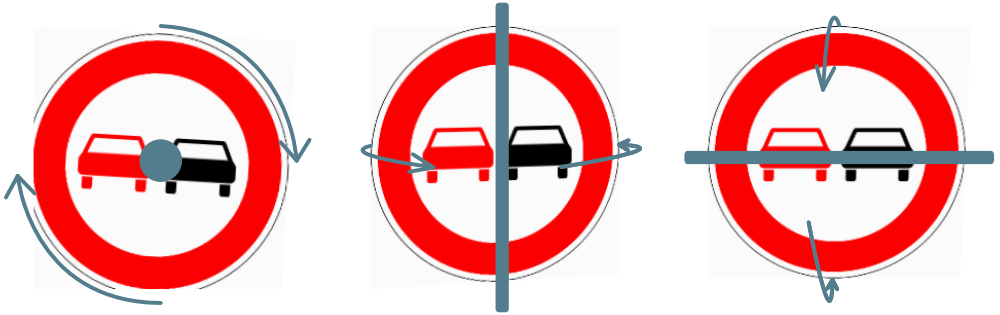
\includegraphics[width=0.6\textwidth]{../images/3 Konzeption des Generative Adversarial Networks/Datenaugmentation/Rotation.png}
	\caption{Rotation der Straßenschilder mittels eulerscher Winkel}
	\label{fig:rotation}
\end{figure}

%\begin{figure}[H]
%    \centering
%    \begin{subfigure}[b]{0.2\textwidth}
%        \centering
%        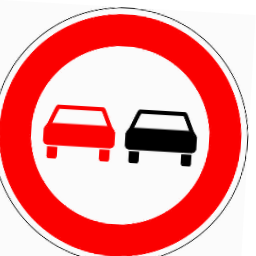
\includegraphics[height=\textwidth]{../images/3 Konzeption des Generative Adversarial Networks/Datenaugmentation/z-axis.png}
%        \caption{Rotation um die z-Achse (\emph{rollen})}
%    \end{subfigure}
%    \hspace{3em}%
%    \begin{subfigure}[b]{0.2\textwidth}
%        \centering
%        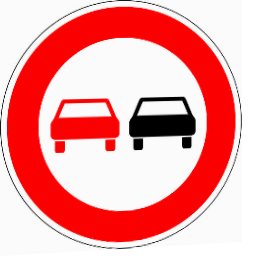
\includegraphics[height=\textwidth]{../images/3 Konzeption des Generative Adversarial Networks/Datenaugmentation/y-axis.png}
%        \caption{Rotation um die y-Achse \emph{}}
%    \end{subfigure}
%    \hspace{3em}%
%    \begin{subfigure}[b]{0.2\textwidth}
%        \centering
%        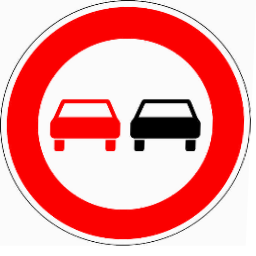
\includegraphics[height=\textwidth]{../images/3 Konzeption des Generative Adversarial Networks/Datenaugmentation/x-axis.png}
%        \caption{Rotation um die x-Achse}
%    \end{subfigure}
%    \caption{Rotationen mittels eulerscher Winkel}
% \end{figure}

Jede Rotation ist durch einen einzelnen Winkel um die jeweilige Achse bestimmt. Kombiniert man die Rotationen, kann die resultierende Tranformation somit durch drei Winkel $(\alpha_z, \alpha_y, \alpha_x)$ eindeutig beschrieben werden. Für die Erzeugung einer zufälligen Rotation müssen randomisierte Werte für diese Winkel bestimmt werden. \cite{math-primer}

Zusätzlich zu der Rotation, soll das Modell die Piktogramme zufällig in ihrer Größe skalieren. Die genannten Augmentationen dienen dazu, die Verteilung der real aufgenommenen Schilder abbilden zu können. Im Datensatz besitzen die Schilder eine unterschiedliche Größe und sind aus verschiedenen Perspektiven aufgenommen. Dadurch dass die Augmentation deterministisch ist, kann sie dazu genutzt werden, um gezielt nur Bilder durch das Modell zu generieren, die aus bestimmten Perspektiven und mit festgelegten Größen generiert wurden. Alternativ kann auch die randomisierte Augmentation beibehalten werden, um eine möglichst große Bandbreite an unterschiedlichen Bildern zu erzeugen.

%Eine Rotation in x- und y-Richtung besitzt folgende sogenannte \emph{Transformationsmatrix} \cite{geometric-ops}:

%\begin{equation}
%    \begin{bmatrix}
%        \cos{\theta} & -\sin{\theta} & 0\\
%        \sin{\theta} & \cos{\theta} & 0\\
%        0 & 0 & 1
%    \end{bmatrix}
%\end{equation}

%Um ein Bild zu Rotieren, multipliziert man in der homogenen Darstellung jeden Pixel des Bilds mit dieser Matrix. Die Winkel $\theta$ sollten alle gleich groß sein, damit das Bild durch die Rotation nicht verzerrt wird. Für die Rotation der Piktogramme der Straßenschilder wird diese Matrix um eine Rotation in z-Richtung erweitert. Die vollständige Gleichung sieht damit wie folgt aus:

%\begin{equation}
%    \begin{bmatrix} \tilde{x} \\ \tilde{y} \\ \tilde{z} \end{bmatrix}
%    =
%    \begin{bmatrix}
%        \cos{\theta_{xy}} & -\sin{\theta_{xy}} & 0\\
%        \sin{\theta_{xy}} & \cos{\theta_{xy}} & 0\\
%        0                 & \sin{\theta_{z}} & 1
%    \end{bmatrix}
%    \cdot \begin{bmatrix} x \\ y \\ 1 \end{bmatrix}
%\end{equation}

%Die linke Seite der Gleichung zeigt $\tilde{p}$, das Ergebnis der Rotation im dreidimensionalen Raum. Die Rotationsmatrix wird dafür mit der homogenen Darstellung des zweidimensionalen Punktes $p$ multipliziert. Die letzte Zeile der Rotationsmatrix stellt die Rotation in z-Richtung dar. Der Term $\sin{\theta_{z}}$ verändert die Pixelwerte in y-Richtung, das heißt das Piktogramm wird in z-Richtung geneigt. Rückblickend wäre jedoch auch eine Rotation in x-Richtung sinnvoll. Dadurch würde der Effekt entstehen, das Foto sei von der Seite aufgenommen worden. Die Rotation der Piktogramme in z-Richtung soll weitaus subtiler sein als in x- und y-Richtung. Deshalb ist $\theta_{z}$ allgemein kleiner als $\theta_{xy}$. \cite{geometric-ops}

%Für die programmatische Implementierung der Rotation mit dem Framework OpenCV muss die Überführung des Bildes aus der homogenen Darstellung zurück in den zweidimensionalen Raum nicht manuell erfolgen. Deshalb soll darauf nicht weiter eingegangen werden. Grundsätzlich wäre dies jedoch der nächste Schritt, um das rotierte Schild in einem zweidimensionalen Bild darstellen zu können.

%\begin{listing}[H]
%    \caption{Rotation der Piktogramme mit OpenCV}
%    \begin{minted}[fontsize=\footnotesize, linenos, breaklines, autogobble]{python}
%        def apply_3d_rotation(img_tensor, theta_xy, theta_z, image_size):
%            """
%            Rotate the img_tensor in x, y and z direction.
%            """
%            transformation_matrix = np.array([
%                [np.cos(theta_xy), -np.sin(theta_xy), 0],
%                [np.sin(theta_xy),  np.cos(theta_xy), 0],
%                [0,                 np.sin(theta_z),  1] 
%            ])
%            rotated_image = cv2.warpPerspective(img_tensor.numpy(), transformation_matrix, (image_size, image_size))
%            return rotated_image
%    \end{minted}
%\end{listing}

%\begin{lstlisting}[language=Python, caption={Rotation der Piktograme mit OpenCV}]
%def apply_3d_rotation(img_tensor, theta_xy, theta_z, image_size):
%    """
%    Rotate the img_tensor in x, y and z direction.
%    """
%    transformation_matrix = np.array([
%    [np.cos(theta_xy), -np.sin(theta_xy), 0],
%    [np.sin(theta_xy),  np.cos(theta_xy), 0],
%    [0,                 np.sin(theta_z),  1] 
%    ])
%    rotated_image = cv2.warpPerspective(img_tensor.numpy(), transformation_matrix, (image_size, image_size))
%    return rotated_image    
%\end{lstlisting}

\section{Training}
Das Training basiert auf den in Kapitel \ref{chap:GANs} vorgestellten Verlustfunktionen für \acp{CycleGAN}. In Abbildung \ref{fig:training} sind hierfür die drei Trainingsschritte des \ac{CycleGAN} dargestellt. Die ersten beiden Schritte berechnen den \emph{Adversarial Loss} von Generator $G$ und Diskriminator $D_y$, beziehungsweise von Generator $F$ und Diskriminator $D_X$. Was hier trainiert wird, ist die Übersetzung von Domäne X in Y, beziehungsweise von Domäne Y in X. Im Anschluss daran erfolgt die Berechnung des \emph{Cycle Consistency Loss}. Das ist der Trainingsschritt der überprüfen soll, dass die von Generator $G$ erzeugten Bilder das erwartete Straßenschild zeigen. Dazu erzeugt $G$ aus einem Piktogramm das Bild eines Straßenschilds woraus $F$ wiederum das Piktogramm erzeugen soll. Der Generator $G$ ist hierbei grün hervorgehoben, da dies das einzige \ac{KNN} ist, dass für die praktische Generierung von Bildern verwendet wird. Die weiteren \acp{KNN} sollen lediglich den Generator $G$ trainieren. \cite{cycleGAN}

\begin{figure}[h]
	\centering
	\includegraphics[width=0.5\textwidth]{../images/3 Konzeption des Generative Adversarial Networks/Training/traffic_signs.png}
	\caption{Trainingsschritte des \ac{CycleGAN}}
	\label{fig:training}
\end{figure}

Für bestimmte Anwendungsfälle schlägt das \ac{CycleGAN} Paper vor, einen \emph{Identity Loss} hinzuzufügen. Dabei wird Generator $G$ ein echtes Bild eines Straßenschilds und Generator $F$ ein echtes Bild eines Piktogramms zugeführt. Da das Eingabebild für $G$ und $F$ bereits aus der Zieldomäne entstammt, wird hier von den Generatoren erwartet, dass sie das Eingabebild möglichst wenig verändern. Die Veröffentlichung schlägt das vor, wenn die Generatoren beispielsweise die Farben der Eingangsbilder beibehalten sollen. \cite{cycleGAN}

Die Vermutung ist, dass der Identity Loss auch für diese Studienarbeit sinnvoll sein kann. Hierdurch könnte das Netzwerk dazu gebracht werden, das Straßenschild möglichst wenig zu verformen und es könnte aus den Eingabebildern erlernen, verschiedene Hintergründe um die Schilder zu erzeugen. Deshalb wird der Identity Loss in diesem Projekt erprobt. Eine Veröffentlichung deutet außerdem darauf hin, dass der Identity Loss die allgemeine Qualität der generierten Bilder verbessern kann \cite{identity-loss}. \cite{cycleGAN}

Zusätzlich schreiben die Autoren der \ac{CycleGAN} Veröffentlichung, dass es sinnvoll sein kann, den \emph{Adversarial Loss} mit einer $\mathcal{L}_2$ Verlustfunktion zu berechnen statt mit einer Binary Crossentropy Verlustfunktion. Das soll das Training stabilisieren. Die pix2pix-Veröffentlichung erwähnt das ebenfalls \cite{pix2pix}. Streng genommen handelt es sich dabei dann bei den Paaren $G$ und $D_y$, beziehungsweise $F$ und $D_x$ nicht mehr um klassiche \acp{GAN}, sondern um sogenannte \emph{least squared \acp{GAN} (LS-GANs)}. In dieser Studienarbeit soll das Training zunächst mit einer klassischen \ac{CycleGAN} Architektur erfolgen. Zeigt sich ein instabiles Training, soll getestet werden, ob sich das Training mittels $\mathcal{L}_2$ Verlustfunktionen stabilisieren lässt. \cite{cycleGAN}

Das Training gilt als beendet, wenn die Verlustfunktionen des Modells gegen einen Wert konvergieren. Um das zu messen, ist eine Form des \emph{Loggings} notwendig. Es müssen demnach über den Verlauf des Trainings die Werte der Kostenfunktionen gespeichert werden. 